%\addbibresource{/home/jorgsk/Dropbox/phdproject/bibtex/jorgsk.bib}
\SUBSECTION{Kinetic model of initial transcription}
Our model describes the process of initial transcription by considering the
following reactions: i) the NAC ii) backtracking iii) unscrunching and abortive
RNA release (UAR), and iv) promoter escape (\FIG~\ref{fig:model_and_rates}).
We refer to backtracking here only as the first unscrunching step, also known as
backstepping. We find the rate constant of backtracking using APs calculated
from experimental data \cite{hsu_quantitative_1996}. The method relies on two
key points. The first is that the reactions of the NAC and backtracking are in
kinetic competition (\FIG~\ref{fig:model_and_rates}). The second is the
assumption that the probability to backtrack at any given template position is
equal to the AP at that position. In combination, we get
\begin{equation*}
    \frac{b_i}{b_i + \text{NAC}_i} = \text{AP}_i,
\end{equation*}
where subscript $i$ indicates position, and NAC and $b$ are the rate constants
of the nucleotide addition cycle and backtracking, respectively. From this
expression, we obtain an expression for the rate constant for backtracking:
\begin{equation}
  b_i = \frac{\text{NAC}_i\cdot\text{AP}_i}{1-\text{AP}_i}.
  \label{eq:backtrackingcalc}
\end{equation}
\FIG~\ref{fig:param_estimation_scheme} contains an example calculation of rate
constants of backtracking when NAC = 10 $s^{-1}$.

We present a rationale for why APs calculated from abundance of aborted RNA
give a good indication of the probability of the initial backtracking step.
The alternative would be that RNAP could backtrack without
producing an abortive RNA, by entering and remaining in long backtracked
pauses, as has been observed for elongating complexes
\cite{shaevitz_backtracking_2003}. In the data we use for rate constant
estimation, GreB was specifically included in the experiments to avoid long
backtracked pauses, and no such pauses were reported
\cite{revyakin_abortive_2006}. Additionally, it is likely that the shortened
RNA-DNA hybrid and strain from scrunching make backtracked initial
transcribing complexes far less stable than their elongating counterparts. We
therefore find it reasonable to assume that once backtracking has commenced in
initial transcription, an abortive RNA is eventually released. Another
possibility is that abortive RNAs can be released instantly without
backtracking via hyper forward translocation. However, this has only been
described for long abortive transcripts ($>$~16 nt) in N25 promoter mutation
variants \cite{chander_alternate_2007, chander_mechanisms_2015}. Since native
N25's abortive RNAs are shorter than 12 nt \cite{chander_alternate_2007}, we
assume that hyper forward translocation does not take place during initial
transcription on native N25 and that backtracking is the only mechanism
leading to the release of an abortive RNA.

In this work we use both APs obtained for the absence of GreB (-GreB) and in
the presence of GreB (+GreB). When GreB is present, backtracked complexes may
be rescued by GreB stimulated cleavage of the unaligned 3\ppp end of the
transcript. Therefore, APs obtained in the presence of GreB represent the
combined probability of both backtracking and avoiding rescue by GreB until
RNA is released. We therefore assume that when GreB is present, GreB-mediated
cleavage and subsequent NACs are rapid steps compared to unscrunching; this is
supported by the finding that unscrunching and abortive RNA release are slow
relative to NAC \cite{revyakin_abortive_2006, margeat_direct_2006}. This
permits using the APs obtained in the presence of GreB as effective
backtracking probabilities. The +GreB AP values used in this work are obtained
from Figure 4B in Hsu et al. \cite{hsu_initial_2006}, and -GreB AP values have
been calculated directly from raw data used to build Table 1 in Hsu et al.\
\cite{hsu_initial_2006} (data provided by Lilian M. Hsu). AP values in Hsu et
al.\ have been obtained in the presence of $100\ \mu M$ NTP at 37 $^{\circ}$C
\cite{hsu_initial_2006}.

\SUBSECTION{Implementation and rate constant estimation}
A central result in this work is the estimation of the rate constants of initial
transcription. We perform this estimation by running multiple simulations with
different combinations of rate constants and evaluating the fitness of each
combination to experimental data. The data used for rate constant estimation
is the distribution of time spent in abortive cycling on the N25 promoter
determined by Revyakin et al.\ \cite{revyakin_abortive_2006}. This data was
obtained under $100\ \mu M$ NTP at 34 $^{\circ}$C, near-identical conditions
to how the APs were obtained \cite{hsu_initial_2006}.

The experimental data was obtained from 100 individual initial transcription
events \cite{revyakin_abortive_2006}. For experiments with single molecules,
there is an inherent stochastic component in the experimental outcome that
derives from the randomness of molecular motion. That this is evident for
transcription can be inferred from the large variation in the speed of
transcription elongation observed in single-molecule experiments
\cite{adelman_single_2002, tolic-norrelykke_diversity_2004}. To account for
this randomness, we perform the kinetic simulations using the Gillespie
algorithm for stochastic simulations of chemical reactions
\cite{gillespie_exact_1977}. Specifically, we make use the version implemented
by Maarleveld et al.\ in the StocPY software \cite{maarleveld_stochpy:_2013}.

The procedure for rate constant estimation (illustrated in
\FIG~\ref{fig:param_estimation_scheme}) is as follows (rate constant names
are given in \FIG~\ref{fig:model_and_rates}): First, we assign random values
to the three rate constants NAC ($k_n$), promoter escape ($k_e$) and
unscrunching and abortive RNA release ($k_u$) within certain fixed boundaries
(see below). These values are chosen independently from a uniform
distribution. Second, we use the rate constant of the NAC and APs to
calculate the rate constant of backtracking ($k_b$) using
Eq.~(\ref{eq:backtrackingcalc}). We then simulate 100 initial transcription
events and calculate the distribution of time spent in abortive cycling as a
result of these specific rate constants. The result is measured against the
empirical distribution \cite{revyakin_abortive_2006} using the root mean
square error. By repeating this procedure several times, we obtain statistics
of which values of rate constants are associated with the best match with
the experimental data. By virtue of using stochastic simulations, one does not
arrive at a unique set of rate constants that have optimal fit with data; if a
simulation is repeated with identical rate constants, slightly different
results will be obtained due to the inherent stochasticity of the reaction
process. Therefore, we identify the best-fitting rate constants from peak of
the fitness distribution, i.e.\ identify those rate constants that stand out
by most often giving the best fit to data.

The boundaries of the rate constants for parameter estimation were chosen from
extrema estimated from experimental findings. The speed of the NAC during initial
transcription cannot be much less than 3 nt/s, since Revyakin et al.\ measured
2.5 seconds as the shortest duration of abortive cycling
\cite{revyakin_abortive_2006} to cover the $\sim 11$ nts required for promoter
escape on N25. At the same time, it should not be larger than 25 nt/s,
which is above the upper limit of what has been measured for transcription
elongation \cite{bai_mechanochemical_2007}. While it is not clear how
transcription would proceed faster for promoter-bound RNAP, we use 25 nt/s as
a maximum value also in order to see if the model is able to discard these
extreme values during rate constant estimation. For backtracking and abortive
RNA release, it is known that the rate constant must be faster than 1
s$^{-1}$, since this was the time-resolution of experimental equipment which
could not resolve this value \cite{revyakin_abortive_2006}. To explore
possible values for all rate constants equally, we set the minimum and maximum
values of all rate constants to be 1 s$^{-1}$ and 25 s$^{-1}$, respectively. 

\begin{figure}[h]
    \begin{center}
      
\includegraphics{../illustrations/model_and_rates_mini}
    \end{center}
  \caption{{\bf Kinetic model of initial transcription on the N25 promoter.}
    From the open complex (OC) transcription proceeds by NACs from one initial
    transcribing complex (ITC) to the next, where each ITC is identified in
    subscript by the length of its nascent RNA. Initial transcription proceeds
    until the nascent RNA has reached the experimentally obtained maximum size
    of abortive transcript; for N25, this is 11 nt \cite{hsu_initial_2006}.
    For ITCs with an RNA of 2 nt in length or longer, there is a competition
    between the NAC and backtracking. Backtracking causes termination of
    transcription, and only further backtracking (unscrunching) and abortive
    RNA release may follow, returning RNAP to the open complex. From the open
    complex, forward transcription may resume once more. The names of the rate
    constants are as follows: $k_n$ (NAC), $k_e$ (promoter escape), $k_u$
    (unscrunching and abortive RNA release) and $k_{b,i}$ (backtracking).}
    \label{fig:model_and_rates}
\end{figure}

\begin{figure}[h]
    \begin{center}
      \includegraphics{../illustrations/parameter_estimation_scheme}
    \end{center}
  \caption{ {\bf Rate constant estimation protocol.} \textbf{1:}
    Rate constants for the NAC, UAR and promoter escape are randomly sampled
    from a uniform distribution (example values are shown). Of these values,
    the NAC is used further to obtain backtracking rates at each template
    position (\textbf{3}). This is done by solving
    Eq.~(\ref{eq:backtrackingcalc}), where the APs are obtained from Hsu et
    al.\ \cite{hsu_initial_2006} (\textbf{2}). The backtracking rate
    constants, together with the NAC, UAR, and promoter escape rate constants
    sampled in step \textbf{1}, encompass the complete kinetic scheme of
    initial transcription (\textbf{4}). This scheme is then used to simulate
    the kinetics of 100 initial transcription events; from these 100 events
    the distribution of time spent in abortive cycling is calculated and
    compared to measured data from Revyakin et al.\
    \cite{revyakin_abortive_2006} (\textbf{5}). From the distance between the
    measured distribution and the simulated distribution, a fitness score is
    produced. This score is associated to the three randomly selected rate
    constants in step \textbf{1}, and is a measure for how well the kinetic
    scheme (the three random rate constants and the AP values) agree with the
    experimental data. By repeating steps \textbf{1}-\textbf{5} multiple
    times, distributions are obtained from where we find which values of the
    rate constants provide the best fit with experimental data.}
    \label{fig:param_estimation_scheme}
\end{figure}
